\documentclass[journal]{IEEEtran/IEEEtran}
\usepackage{algorithm2e}
\usepackage{cite}
\usepackage[square,numbers]{natbib}
\usepackage{filecontents,lipsum}
\usepackage{subcaption}
\usepackage[skip=2pt,font=scriptsize]{caption}
\usepackage[skip=2pt,font=scriptsize]{subcaption}
\usepackage{amsmath,amssymb,amsfonts}
\usepackage{algorithmic}
\usepackage{graphicx}
\usepackage{tabularx}
\usepackage{multirow}
\usepackage{textcomp}
\usepackage{color}
\usepackage{cite}
\usepackage[colorlinks,bookmarks=false,citecolor=blue,linkcolor=blue,urlcolor=blue]{hyperref}
\def\BibTeX{{\rm B\kern-.05em{\sc i\kern-.025em b}\kern-.08em
    T\kern-.1667em\lower.7ex\hbox{E}\kern-.125emX}}

\ifCLASSINFOpdf


\fi
\hyphenation{op-tical net-works semi-conduc-tor}
% updated with editorial comments 8/9/2021

\begin{document}

\title{Dynamics of a Memristive Autapse-Synapse Neural Network: Application to Medical Image Encryption}
%\title{Dynamics of Memristive Autapse-Synapse Neural Network Model and its Application to Medical Cryptography}

\author{Xi Zhang, Donghua Jiang,  Jean De Dieu Nkapkop, Zeric Tabekoueng Njitacke, Musheer Ahmad,  Liya Zhu, Nestor Tsafack,

\thanks{Manuscript received ****; revised ****}
%\thanks{This work is partially funded by the Polish National Science Center under the Grant OPUS $14 No.2017/27/B/ST8/01330$.}

\thanks{Xi Zhang is with the chool of Aeronautics Engineering, Air Force Engineering University, Xi'an 710038,China}

\thanks{Donghua Jiang is with the School of Computer Science and Engineering, Sun Yat-sen University, Guangzhou 511400, China}

\thanks{Jean De Dieu Nkapkop is with the Department of Electrical Engineering and Industrial Computing, University Institute of Technology, P.O. Box 8698 Douala, Cameroon}

\thanks{Zeric Tabekoueng Njitacke is with the Department of Electrical and Electronic Engineering, College of Technology (COT), University of Buea, P.O. Box 63, Buea, Cameroon and Department of Automation, Biomechanics and Mechatronics, Lodz University of Technology, Lodz, Poland}

\thanks{Musheer Ahmad is with the Department of Computer Engineering, Jamia Millia Islamia, New Delhi 110025, India}

\thanks{Nestor Tsafack is with the Research Unit of Laboratory of Energy and Artificial Intelligence (RU-LEAI), Electrical Engineering Department and Industrial Computing of ISTAMA, University of Douala, P.O. Box 3223, Douala, Cameroon}

\thanks{Xingyuan Wang is with the School of Information Science and Technology, Dalian Maritime University, Dalian 116026, China}
}
\markboth{IEEE Transactions on Medical Imaging}%,~Vol.~14, No.~8, August~2015}%
{Shell \MakeLowercase{\textit{et al.}}: Bare Demo of IEEEtran.cls for IEEE Journals}

%\IEEEpubid{0000--0000/00\$00.00~\copyright~2021 IEEE}
% Remember, if you use this you must call \IEEEpubidadjcol in the second
% column for its text to clear the IEEEpubid mark.

\maketitle

\begin{abstract}
With the advent of the physical memristor, various memristive neural network models have been designed and analyzed to mimic some human brain functions. However, there is a realistic issue because many works reported the coupling of neuron models using either memristive synapse or memristive autapse, whereas in the real brain, a neuron can interact with both another neuron (memristive synapse) and with itself (memristive autapse). Two main ideas are developed in this work. First, we investigate the dynamics of two different neurons coupled via memristive synapse and memristive autapse. The analyses indicate that the global dynamics of this highly relies on the neuron's coupling strength. Second, a cryptographic scheme based on both S-box driven block compressive sensing and the memristive autapse synapse model is proposed. Performance analyses indicate that the coupling strength of the proposed neural network model can be adjusted to increase or decrease the security of medical data
 \end{abstract}

\begin{IEEEkeywords}
Memristive synapse; Memristive autapse; Neural network model; Compressive sensing; Image encryption.
\end{IEEEkeywords}

\section{Introduction}
\label{intro}
\IEEEPARstart{N}{}eurons are brain cells that are used to transmit information. They are all interconnected and communicate with each other by electrical and chemical messages through branches called dendrites on which the axons end to transmit information. Neurons are responsible of several functions of the human brain. The complexity of the brain has encouraged scientists to study neuronal dynamics \cite{sung2022simultaneous}. Thus, in the early 1980s, artificial neuron models and artificial neural network models emerged, including but not limited to the Hodgkin-Huxley neuron model (HH) \cite{abbott1990model}, FitzHugh-Nagumo (FHN) neuron model \cite{nouri2015digital}, Morris-Lecar neuron model (ML) \cite{song2019autapse}, Hindmarsh-Rose neuron model (HR) \cite{cai2021smooth}, Chay neuron model \cite{xu2020bifurcations}, Hopfield neural network (HNN) \cite{bao2019dynamical} and the Cellular neural network (CNN) model \cite{tlelo2022optimization}. The analysis of the dynamics of these models made it possible to reveal several electrical activities in the brain dynamics such as periodic spiking, periodic bursting, and mode transition \cite{njitacke2021window}. Although these classical models have allowed the demonstration of some dynamic behaviors of the brain, it is quite obvious that the human brain is very complex. Some researchers believe that the coupling of neurons may be more realistic in highlighting the dynamic behaviors of the human brain. Mohammad and collaborators exploited gap junction with different coupling strengths to link type I and type II excitability neurons \cite{razvan2020emergence}. The investigations indicated that the coupling strength considerably affects the dynamics of the neurons. The discovery of the physical memristor reactivated interest on neural networks dynamic analysis. It should be noted that the memristor has several properties including, programmability, memorability, and its nonlinearity. These properties can be exploited to reproduce the synaptic functions of the human brain, such as plasticity. It is important to stress that the memristor can also be exploited to show the effect of electromagnetic radiation on the electrical activity of the neuron. Consequently, several researchers believe that with the memristor as a neuronal synapse or autapse, the dynamic of the artificial neuron is more realistic and much research can be identified in this line \cite{lin2021review}. A review on chaos in the dynamics of coupled neurons has been investigated by Hairong and collaborators \cite{lin2021review}. In this review, it is obvious that memristive autapse can be exploited to interconnect the dendrites and the axon of the same neuron. On the other  hand, a  memristive synapse is used to couple two identical neurons or two different neurons. Note that the analysis of coupled neurons using both memristive autapse and memristive synapse has not yet been reported. Tabekoueng and colleagues used a memristive synapse to connect a FitzHugh-Nagumo (2-D) neuron to a  Hindmarsh-Rose (3-D) neuron \cite{njitacke2022hamilton}. The dynamics reveals the coexistence of infinite patterns in the state space. \cite{tan2020simple} exploited a new locally active memristor as synapse to couple neurons. It can be observed that with the advent of the memristor, the field of neurodynamics has made significant progress. However, it is obvious to note that none of the most recent works has investigated the dynamics of coupled neurons using both memristive synapse and memristive autapse. This limitation is our main motivation in the design of the new neuronal model presented in this work. \\
Security in communication channels is one of the primary concerns of a very large scientific community. One of the most affected areas is the medical field, where highly sensitive medical information can pass from sender to receiver. These confidential data must be secured. In this perspective, several algorithms for securing medical images can be identified in the literature \cite{parameshachari2022medical,njitacke2021complex}. \cite{parameshachari2022medical} exploited the SCAN technique and Tent map in chaotic windows to secure medical images. The method decomposes the image planes into bit first, followed by a pixel rearrangement and finally a diffusion process. Njitacke and collaborators recently studied the electromagnetic effect of two coupled neurons on the security of medical images \cite{njitacke2021complex}. The compressed sensing technology is used to compress the image to fit its size with the communication channel bandwidth. The results provided secured and compressed output images. It should be noted that the compression performance in compressive sensing mainly relies on the construction of measurement matrix. In this work, the measurement matrix is constructed using the S-box with nonlinear and pseudorandom properties generated from the sequences of the memristive autapse-synapse neural network model. This idea is completely new. The main objective of this work can be summarized in the sequel:

\begin{enumerate}
\item  Couple two different neurons to form a neural network and analyze its dynamics in terms of coupling strength using memristive autapse and synapse.The most noteworthy point is that the idea of coupling neurons using both memristive synapse and autapse is completely new and not yet studied in the literature.
\item Exploit the output of the memristive autapse-synapse neural network model to construct a new S-box with strong nonlinearity and pseudo-random properties.
\item Using the generated S-box, create a robust and hardware-friendly compressive sensing model (suitable for practical application). It should be noted that this concept has not yet been reported in previous works. Meanwhile, it opens up a new application scenario for the S-box.
\item Develop a compression-encryption scheme for medical data that incorporates the designed compressive sensing model as well as the memristive autapse-synapse neuron model; and evaluate the effect of the memristive synapse-autapse neural network coupling strength on the security of the medical data. 
\end{enumerate} 
This paper is arranged in the following sections in addition to the introductive Section \ref{intro}. The construction method of the proposed memristive autapse-synapse neural network is presented in Section \ref{dm}. Its dynamics is analyzed with the help of some well-known tools. Section \ref{sec3} describes the designed method of the s-box using the memristive autapse-synapse neural network. In Section \ref{sec4} the compressive sensing encryption based on the memristive autapse-synapse neural network is presented with the results. Finally, the work is summarized in Section \ref{con}.




\section{The memristive autapse-synapse neuron model}
\label{dm}
\subsection{Model description}

The memristor is the fourth missing electronic component, beside the inductor, the capacitor, and the resistor. It is mainly characterized by its capability to save information, given that its resistance changes from a very large value to a very low value, which is interpreted as '1' and '0' logics. As such, the memristor is a suitable tool to reproduce the dynamics of the human brain. A novel memristor model is introduced in this work to couple neurons, and the corresponding mathematical equation is defined by Eq.\ref{eq1}.

\begin{equation}\label{eq1}
\left\{ \begin{array}{l}
 i = G(w)\upsilon  = \alpha w\upsilon  \\ 
 \frac{{dw}}{{dt}} = g(w,\upsilon ) = \gamma \upsilon  + \beta \cos (w) \\ 
 \end{array} \right.
\end{equation}

In Eq.\ref{eq1}, the term $G(w)$  represents the memductance of the memristor, while $g(w,\upsilon )$ the evolution of that inner variable of the memristor. By applying various sinusoidal excitation of the form $\upsilon  = A\sin (2\pi Ft)$  on the designed memristor with  $\alpha  = 0.1$,  $\beta  = 1$,  $\gamma  = 0.2$, the pinched hysteresis loop in the voltage-current plane of the memristor is established (Fig.\ref{fig1}). Consequently the memristor model is suitable to design memristive synapse-autapse neuronal models. 

\begin{figure}[!t]
	\centering
	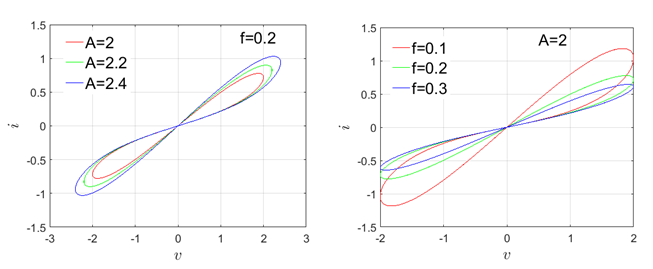
\includegraphics[width=0.5\textwidth]{fig1.png}
		\caption{Hysteresis representation of the proposed memristor exploited for autapse-synapse.}
	\label{fig1}
\end{figure}

Neuronal models that are able to reproduce human brain dynamics have greatly improved the field of neurodynamics. Various models have been introduced and analyzed to show some common dynamics in the human brain. Hindmarsh and Rose (HR) designed one of the most simple and single neuron model capable to display most of firing activities in the human brain. The mathematical description of Hindmarsh-Rose neuron model includes both 2-D and 3-D models. 2-D model is described by Eq.\ref{eq2} and is quite simple than the 3-D model.

\begin{equation}\label{eq2}
\left\{ \begin{array}{l}
 {{\dot x}_1} = {y_1} - {a_1}x_1^3 + {b_1}x_1^2 + {I_1} \\ 
 {{\dot y}_1} = {c_1} - {d_1}x_1^2 - {y_1} \\ 
 \end{array} \right.
\end{equation}

Another classical neuronal model presented and analyzed in the literature is the FitzHugh–Nagumo (FHN) model. This model is introduced by simplifying the Hodgkin and Huxley (HH) neuronal model. The FHN neuron model (presented in Eq.\ref{eq3}) also reflects some well-known dynamical behavior present in the human brain.

\begin{equation}\label{eq3}
\left\{ \begin{array}{l}
 {{\dot x}_2} = {x_2} - {d_2}x_2^3 - {y_2} + {I_2} \\ 
 {{\dot y}_2} = {c_2}({a_2} + {x_2} - {b_2}{y_2}) \\ 
 \end{array} \right.
\end{equation}

Human brain is made of different interconnected neurons. However most of the recent works in the literature proposed and analysed the interconnection of identical neurons. Also note that the recent works in the literature shows the interconnection of neurons using either memristive autapse or memristive synapse. In this work the 2-D HR model described by Eq.\ref{eq2} and the 2-D FHN model described by Eq.\ref{eq3} are exploited to design the memristive autapse-synapse neural network model as described by Eq.\ref{eq4} following the synoptic representation of Fig\ref{fig}. 

\begin{equation}\label{eq4}
\left\{ \begin{array}{l}
 {{\dot x}_1} = {y_1} - {a_1}x_1^3 + {b_1}x_1^2 + {I_1} - \alpha {w_2}({x_1} - {x_2}) - \alpha {w_1}{x_1} \\ 
 {{\dot y}_1} = {c_1} - {d_1}x_1^2 - {y_1} \\ 
 {{\dot w}_1} = \gamma {x_1} + \beta \cos ({w_1}) \\ 
 {{\dot x}_2} = {x_2} - {d_2}x_2^3 - {y_2} + {I_2} + \alpha {w_2}({x_1} - {x_2}) \\ 
 {{\dot y}_2} = {c_2}({a_2} + {x_2} - {b_2}{y_2}) \\ 
 {{\dot w}_2} = \gamma ({x_1} - {x_2}) + \beta \cos ({w_2}) \\ 
 \end{array} \right.
\end{equation}

Note that such model better reflects the real dynamics of the neurons in human brain. The coupling method of the neurons follows the Campbell and Waite principle [1]. In this model ${x_i}$  represent the fast variable or the potential membrane and   indicate the slow variable or the ion current (Na+ or K+). ${w_i}$  stand for the inner variable of the memristive autapse as well as the memristive synapse.  $\alpha $, $\beta$  and $\gamma $  represent the parameters of the memristive synapse and autapse.  ${a_i}$,  ${b_i}$,  ${c_i}$, ${I_i}$  and ${d_i}$  are traditional parameter of the neuron model defined by Eq.\ref{eq5} for invariant parameters.

\begin{figure}[!t]
	\centering
	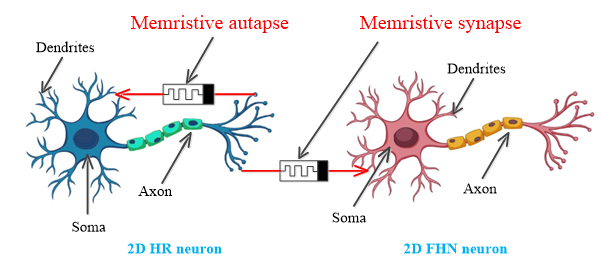
\includegraphics[width=0.5\textwidth]{fig.png}
		\caption{Synoptic representation of the coupling principle though memristive synapse and autapse.}
	\label{fig}
\end{figure}

\begin{equation}\label{eq5}
\left\{ \begin{array}{l}
 {a_1} = 1;{\rm{    }}{b_1} = 3;{\rm{   }}{c_1} = 1;{\rm{   }}{d_1} = 5 \\ 
 {a_2} = 1;{\rm{  }}{b_2} = 0.1;{\rm{ }}{c_2} = 0.1;{\rm{ }}{d_2} = 1/3 \\ 
 \end{array} \right.
\end{equation}

\subsection{Dynamics of the memristive autapse-synapse neural network model}

Remember that a brain-like complex system is made up of a large number of neurons that are linked together. These neurons are important in a variety of biological processes, including hearing, speech, memory, emotions, learning, transport, and information processing/coding, to name a few \cite{lin2021review}. Based on a global bifurcation analysis, the complex behaviors of the introduced model can be easily investigated. It should be noted that the investigation of stability of the model revealed that it is equilibrium free, therefore the considered neuron models exhibits hidden Dynamic.

\begin{figure}[!t]
	\centering
	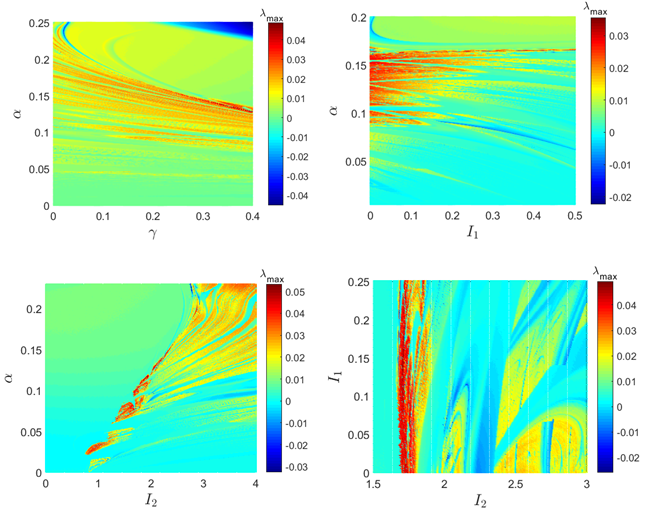
\includegraphics[width=0.5\textwidth]{fig2.png}
		\caption{Two-parameter diagrams obtained when two parameters of the coupled neurons are simultaneously varied. The $(\gamma, \alpha)$ is obtained for $I_{1}=0.1, I_{2}=2.5$. The $\left(I_{1}, \alpha\right)$ is obtained for $\gamma=0.2, I_{2}=2.5$. The $\left(I_{2}, \alpha\right)$ is obtained for $\gamma=0.2, I_{1}=0.1$. And the $\left(I_{2}, I_{1}\right)$ is obtained for $\gamma=0.2, \alpha=0.1$. Initial conditions are $(0.1,0.1,0.1,0.1,0.1,0.1)$.}
	\label{fig2}
\end{figure}

Lyapunov exponent graphs with two parameters are used to quickly explore the global dynamics of the coupled neurons. These graphs are created by jointly increasing two parameters of the coupled neurons from a minimum to a maximum value. The maximum Lyapunov exponent is estimated with the Wolf algorithm \cite{njitacke2022hamilton} at each step of the variation and plotted on the same graph. The two-parameter Lyapunov diagrams of Fig. \ref{fig2} are obtained using the computational method described above. According to the diagrams, several firing activities can be developed by the coupled neurons via the memristive autapse synapse. Among them, it can be found regular behaviors with  ${\lambda _{\max }} \le 0$, and irregular behaviors with  ${\lambda _{\max }} > 0$.  Using the parameters of the fourth two-parameter diagrams as argument (the plane  $\left( {{I_2},{I_1}} \right)$), the bifurcation plot of Fig. \ref{fig3} and the corresponding plot of the maximum Lyapunov exponent have been evaluated.

\begin{figure}[!t]
	\centering
	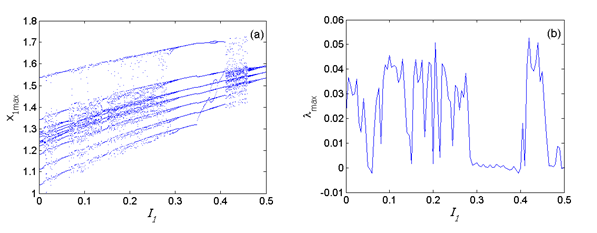
\includegraphics[width=0.5\textwidth]{fig3.png}
		\caption{(a) Bifurcation diagram showing the local maxima of the state variable of the membrane potential of the first neuron versus the extemal current $I_{1}$. The corresponding graph of the maximum Lyapunov exponent is present in (b). These diagrams are obtained for $I_{2}=1.75, \gamma=0.2, \alpha=0.1$. Initial conditions are $(0.1,0.1,0.1,0.1,0.1,0.1)$.}
	\label{fig3}
\end{figure}

From that bifurcation diagram, it is obvious that the dynamic behavior of the coupled neuron when the external current ${I_1}$  of the neuron is varied changes from chaotic to periodic behavior through several chaotic and periodic windows. For some discrete values of ${I_1}$  the chaotic and periodic phase portrait of Fig.\ref{fig4} have been computed to further support the  irregularity and the regularity of the patterns found in the coupled neurons via a memristive autapse-synapse. The Lyapunov exponents corresponding to the chaotic state of Fig.\ref{fig4}-a have been computed. The outcome shows the following values ${\lambda _1} = 0.0525859$, ${\lambda _2} =  - 0.00174098$, ${\lambda _3} =  - 0.227193$, ${\lambda _4} =  - 0.867789$, ${\lambda _5} =  - 1.06122$, ${\lambda _6} =  - 2.98989$. From these values we computed the Kaplan-York dimension (KY) as $DK = 2 + ({\lambda _1} + {\lambda _2})/{\lambda _3}$ and the result produces $DK=2.2237$. This value simply shows that, the attractor in Fig.\ref{fig4}-a presents chaotic state of the memristive autapse-synapse neural network.



\begin{figure}[!t]
	\centering
	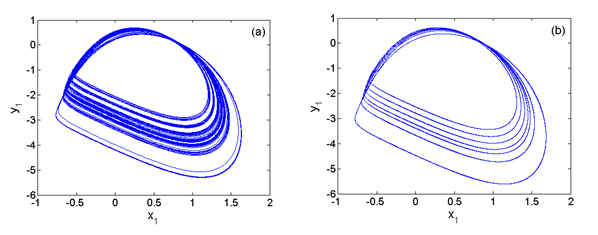
\includegraphics[width=0.5\textwidth]{fig4.png}
		\caption{(a) Chaotic phase portrait obtained for $I_{1}=0.2$ while (b) represents the periodic phase portrait obtained for $I_{1}=0.5$}
	\label{fig4}
\end{figure}

\begin{figure}[!t]
	\centering
	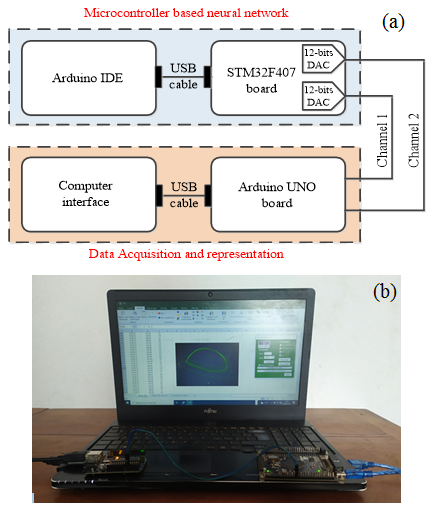
\includegraphics[width=0.5\textwidth]{figg.png}
		\caption{(a) The topology of the Microcontroller implementation. (b) Experimental setup of the proposed neural network model.}
	\label{figg}
\end{figure}

\subsection{Microcontroller Implementation of the neural network}

Two main techniques are usually exploited to implement neural network model namely analogue techniques and digital techniques. Analogue techniques exploit some off-the shell electronic component such as resistors, capacitors, inductors and operational amplifiers to reproduce the dynamics of neural network models. Analogue techniques are very sensitive to temperature variation of the components used. In addition, noise significantly affects the results in this case. Digital techniques use some numerical environment to implement neural network models. Some of the well-known environments include STM board, Arduino board, FPGA board just to name few. In this work STM32F407 and Arduino UNO to implement the neural network model following the synoptic diagram of Fig.\ref{figg}-(a) These boards are low cost and open source microcontroller environments for digital electronic systems and applications. The experimental configuration is given in Fig.\ref{figg}-(b). STM32F407 is used jointly with the Runge-Kutta algorithm to solve the neural network model. Arduino UNO which is connected to the DAC (digital to analogue) pins of the STM32F407 to construct the data acquisition system. A computer interface is used jointly with the acquired data to plot the corresponding phase portrait in real time (Fig.\ref{figgg}).

\begin{figure}[!t]
	\centering
	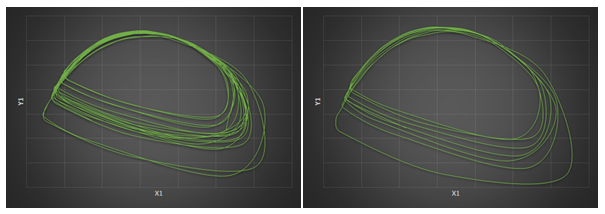
\includegraphics[width=0.5\textwidth]{figgg.png}
		\caption{Experimental phase portrait obtained from the microcontroller implementation of the proposed neural network. These results are obtained using the same values that enable to obtain the results in Fig.\ref{fig2}.}
	\label{figgg}
\end{figure}


\section{Description of newly designed S-box}
\label{sec3}
\subsection{S-box generation algorithm}

This section is concerned with the description of the proposed method with which the optimized S-box gets generated. The proposed S-box method involves two phases. In the first phase, an initial random chaotic S-box is constructed with the help of the proposed memristive synapse-autapse neuron model in Eq. \ref{eq4}. Initial phases make use of random chaotic values to extract integer values lying the domain of ${\rm{8}} \times {\rm{8}}$  S-box. The first occurrence of such integer values is saved in an array. The procedure is repeated until the array has unique 256 elements in  $\left[ {0,{\rm{ }}{2^8} - 1} \right]$. The random nature of S-boxe generated doesn’t guarantee the yielding of strong components \cite{ahmad2018random}. Hence, it is advisable to have some mechanism which can evolve the S-boxes in terms of its security performance. Therefore, an intelligent heuristic is suggested which has the credibility to evolve the composite fitness function in the second phase. The complete method for the optimized S-box generation is presented as Algorithm \ref{algo1}. The fitness function is constructed with an aim to be maximized. The fitness function is composite in the sense that it is based on nonlinearity and differential uniformity of the anticipated S-box. Hence, the maximized fitness value tends to produce S-box with higher nonlinearity and lower differential uniformity as desired. The anticipated fitness function is unique and different as it involves two performance parameters instead of just one. In practice, only nonlinearity is adopted for the performance optimization of the S-box. The fitness function $Fi{t_S}$  considered in the proposed work to evolve the S-box for better security performance has the form of Eq.\ref{eq6}.
\begin{equation}\label{eq6}
Fitness{\rm{ }}function:{\rm{  }}Fi{t_S} = NL(S) + 256 - DU(S)
\end{equation}
\SetKwComment{Comment}{/* }{ */}
\RestyleAlgo{ruled}
\begin{algorithm}
\KwData{Initial parameters of memristive synapse-autapse neuron model parameters; positive integers  $T,{C_{\rm{1}}},{C_{\rm{2}}}$; maximum number of passes  $PAS{S_{max}}$.}
\KwResult{S-box  ${S_{optm}}$.}

\texttt{}

\textbf{\textit{Initialization:}}

\textbf{1.} Take empty array  $SB = {\rm{ }}\left[ {{\rm{ }}\,\,} \right]$; set flag $yes = {\rm{ 1}}$.\\



\textbf{2.} Solve the memristive autapse synapse neuron model in the chaotic range to obtain ${x_1},{y_1},{w_1},{x_2},{y_2},{w_2}$ with $T$ elements and discard all but keep the last state. 



 \While{$yes$}{
	\textbf{3.} Solve the memristive autapse synapse neuron model in the chaotic range to obtain ${x_1},{y_1},{w_1},{x_2},{y_2},{w_2}$.
	  

	        
	\textbf{4.} Compute  $u = {\rm{ }}[{\rm{floor}}({x_1} \times {\rm{1}}{0^{{\rm{14}}}})]{\rm{mod}}\left( {{\rm{256}}} \right)$
  

  
  \If{value $u$  doesn't belong to array  $SB$}{
    append value $u$  in array $SB$
  }
   \If{array $SB$ contains $256$ elements}{
 \textbf{5.}  Set $yes = 0$, and $Fi{t_{SB}} = Fitness\left( {SB} \right)$
   }
}

      \texttt{}
  
\textbf{\textit{Fitness Refinement:}}


  
   \For{$i = {\rm{ 1}}$ to $PAS{S_{max}}$}{
  \textbf{6.} Solve the memristive autapse synapse neuron model in the chaotic range to obtain ${x_1},{y_1},{w_1},{x_2},{y_2},{w_2}$.
  

     
  \textbf{7.} Compute  ${C_{\rm{1}}} = {\rm{ }}[{C_{\rm{1}}} + {\rm{floor}}(x \times {\rm{1}}{0^{{\rm{14}}}})]{\rm{mod}}\left( {{\rm{256}}} \right){\rm{ }} + {\rm{ 1}}$
   

     
  \textbf{8.} Compute  ${C_{\rm{2}}} = {\rm{ }}[{\rm{floor}}(\left( {{x_1} + {y_1}} \right) \times {\rm{1}}{0^{{\rm{14}}}})]{\rm{mod}}\left( {{\rm{256}}} \right)$
   

     
  \textbf{9.} Compute  ${C_{\rm{3}}} = bitxor\left( {SB\left( {{C_{\rm{1}}}} \right),{C_{\rm{2}}}} \right)$
   

     
  \textbf{10.} Find ${C_{\rm{4}}}$  such that $SB\left( {{C_{\rm{4}}}} \right) = {C_{\rm{3}}}$ 
   

     
  \textbf{11.} Exchange $SB\left( {{C_{\rm{4}}}} \right)$  with $SB\left( {{C_{\rm{1}}}} \right)$
   

     
  \textbf{12.} Set  ${S_{optm}} = SB$
   

     
 \textbf{13.} Evaluate fitness of ${S_{optm}}$ as: $Fi{t_{optm}} = Fitness\left( {{S_{optm}}} \right)$   
    

        
   \If{($Fi{t_{optm}} \ge Fi{t_{SB}}$)}{ 
   \textbf{14.} $SB = {S_{optm}}$ and $Fi{t_{SB}} = {\rm{ }}Fi{t_{optm}}$
   }
   }
   
   \textbf{15.} Final S-box is ${S_{optm}}$  with fitness $Fi{t_{optm}}$ 
    
   \caption{Generation of S-box with optimized fitness}\label{algo1}
\end{algorithm}
\subsection{S-box performance analysis}

The security evaluation of the above described S-box is crucial to judge the performance against some well accepted parameters. The S-box method is implemented with the following settings: ${e_0} = 0.123,{\rm{ }}{f_0} = 0.234,{\rm{ }}{g_0} = 0.345,{\rm{ }}a = 3.72,{\rm{ }}b = 0.98$, $t = 0.00001,{\rm{ }}T = 100,{\rm{ }}{C_1} = {C_2} = 34,{\rm{ }}PAS{S_{max}} = 100,000$ . The S-box obtained after executing the Algorithm \ref{algo1} is presented in Table \ref{tab1}. The cryptographic properties of the S-box are assessed by quantifying the performance parameters such as nonlinearity (high is better), differential uniformity (lower is better), SAC (ideal is $0.5$), bits independence criterion (higher is better for NL), and linear approximation probability (lower is better). The following subsections are prepared to analyze the most important of these metrics (Nonlinearity and Differential uniformity) for security evaluation \cite{ahmad2018random}.

\begin{table}
	\centering
	\caption{Generated optimized $8 \times 8$ S-box using Algorithm \ref{algo1}.}
	\label{tab1}
	\resizebox{\columnwidth}{!}{
\begin{tabular}{|*{17}{c|}}
	\hline
	R/C  & 0 & 1 & 2 & 3 & 4 & 5 & 6 & 7 & 8 & 9 & A & B & C & D & E & F \\
	
	\hline
	0  & 187 & 228 & 125 & 50 & 25 & 51 & 150 & 103 & 91 & 136 & 40 & 49 & 121 & 113 & 159 & 153 \\
	
	\hline
	1  & 203 & 235 & 176 & 70 & 253 & 24 & 152 & 138 & 243 & 185 & 54 & 248 & 219 & 207 & 241 & 102 \\
	
	\hline
	2  & 105 & 38 & 168 & 211 & 36 & 5 & 116 & 229 & 88 & 22 & 147 & 14 & 13 & 71 & 80 & 148 \\
	
	\hline
	3  & 36 & 245 & 154 & 66 & 239 & 48 & 162 & 143 & 64 & 142 & 233 & 157 & 193 & 63 & 165 & 220 \\
	
	\hline
	4  & 42 & 21 & 158 & 130 & 39 & 250 & 133 & 244 & 112 & 234 & 173 & 32 & 206 & 114 & 30 & 221 \\
	
	\hline
	5  & 218 & 86 & 124 & 0 & 240 & 52 & 61 & 3 & 180 & 203 & 169 & 84 & 82 & 99 & 177 & 199 \\
	
	\hline
	6  & 126 & 224 & 184 & 255 & 232 & 117 & 144 & 9 & 249 & 31 & 167 & 8 & 4 & 226 & 89 & 155 \\
	
	
	\hline
	7 & 181 & 123 & 175 & 69 & 118 & 79 & 67 & 194 & 145 & 182 & 23 & 237 & 205 & 238 & 96 & 104 \\
	
	\hline
	8 & 172 & 198 & 188 & 65 & 191 & 179 & 171 & 37 & 18 & 149 & 254 & 15 & 230 & 216 & 214 & 7 \\
	
	\hline
	9 & 58 & 156 & 183 & 72 & 87 & 98 & 46 & 146 & 11 & 197 & 33 & 81 & 75 & 222 & 17 & 16 \\
	
	\hline
	A  & 108 & 120 & 29 & 76 & 45 & 44 & 247 & 213 & 60 & 59 & 106 & 95 & 209 & 231 & 164 & 57 \\
	
	\hline
	B  & 137 & 41 & 174 & 2 & 56 & 77 & 68 & 242 & 192 & 140 & 34 & 210 & 195 & 215 & 1 & 132 \\
	
	\hline
	C  & 119 & 212 & 151 & 178 & 111 & 139 & 85 & 201 & 115 & 131 & 246 & 93 & 12 & 189 & 141 & 97 \\
	
	\hline
	D  & 128 & 6 & 47 & 135 & 19 & 78 & 186 & 129 & 94 & 10 & 73 & 62 & 160 & 161 & 166 & 90 \\
	
	\hline
	E  & 26 & 43 & 225 & 170 & 20 & 204 & 100 & 107 & 127 & 27 & 35 & 208 & 223 & 163 & 74 & 83 \\
	
	\hline
	F  & 252 & 110 & 134 & 101 & 122 & 92 & 196 & 109 & 28 & 55 & 251 & 190 & 53 & 227 & 200 & 217 \\
		
	\hline
\end{tabular}
}
\end{table} 

\subsubsection{Nonlinearity}

  Evaluating the nonlinearity transformation of data from the plaintext to the encrypted data is the primary task for an S-box in block cryptosystems. The nonlinearity measure is considered as the most fundamental piece which defines the security and strength of whole system \cite{ahmad2018random}. The strong confusion capability of block cryptosystems is primarily associated with the large nonlinearity to mitigate linear cryptanalysis. The nonlinearity is usualy evaluated with the help of Eq.\ref{eq7}. 

\begin{equation}\label{eq7}
NL(f) = 128 - 0.5\left( {\mathop {\max }\limits_{w \in {{\{ 0,1\} }^8}} \left| {{S_f}(w)} \right|} \right)
\end{equation}

${S_f}\left( z \right)$  indicates the Walsh spectrum of the 8-bit boolean function $f$, which is provided on Eq.\ref{eq8}

\begin{equation}\label{eq8}
{S_f}(w) = \sum\limits_{u \in {{\{ 0,1\} }^8}} {{{( - 1)}^{f(u) \oplus u.w}}} 
\end{equation}

Here, $u.w$ is the bitwise dot product of two 8-bit vectors. In this work the results of nonlinearity are presented in Table \ref{tab2}. The proposed S-box showed a decent nonlinearity behavior as it has minimum NL value ($110$), maximum NL value ($112$) and average NL value ($111.25$). It is evident that all nonlinearity scores are all greather than $110$. This implies that the proposed S-box which is evolved on considered fitness function has admirable ability to bring high nonlinear transformation to oppose related assaults from attackers. 


\begin{table}
	\centering
	\caption{Nonlinearities of Boolean functions of optimized S-box.}
	\label{tab2}
	\resizebox{\columnwidth}{!}{
\begin{tabular}{|c|c|c|c|c|c|c|c|c|c|c|c|}
\hline$f_{i}$ & $f_{0}$ & $f_{1}$ & $f_{2}$ & $f_{3}$ & $f_{4}$ & $f_{5}$ & $f_{6}$ & $f_{7}$ & $\min$ & $\max$ & $a v e r a g e$ \\
\hline$N L\left(f_{i}\right)$ & 110 & 112 & 110 & 112 & 110 & 112 & 112 & 112 & 110 & 112 & $111.25$ \\
\hline
\end{tabular}
}
\end{table}


\subsubsection{Differential uniformity}

The resistivity of S-Box against the differential cryptanalysis (DC) is estimated by differential uniformity. The attack analysis is connected with existing imbalance on the input or output scattering to attack block ciphers and S-boxes. If the EX-OR of each output has identical uniformity with the value of EX-OR of each input contradictorily the cryptanalysis can succeed. On the off chance that an S-box is uniform in input or output distribution, it is supposed to be good resistant to the anticipated differential attack. Therefore, EX-OR table is favored that the highest value of differential uniformity (DU) ought to be just about as little as could really be expected. Meaning, a smaller value of DU indicates the decent ability of the S-box to withstand the DC. For an S-box S, the differential uniformity is measured with Eq.\ref{eq9}: 



\begin{equation}\label{eq9}
DU(S) = \mathop {\max }\limits_{\delta m \ne 0,\delta n} \left( {\# \left\{ {w \in X|S(m) \oplus S(m \oplus \delta m) = \delta n} \right\}} \right) 
\end{equation}

Here, set $X$ holds all probable input values and the size of this set is $256$ for an ${\rm{8 \times 8}}$ S-box. The EX-OR distribution result shows that the biggest value is 8 indicating the capbility of the S-box presented in this work to oppose the differential cryptanalysis.

 

%\begin{table}
%	\centering
%	\caption{EX-OR distribution for proposed S-box.}
%	\label{tab3}
%	\resizebox{\columnwidth}{!}{
%\begin{tabular}{|l|l|l|l|l|l|l|l|l|l|l|l|l|l|l|l|}
%\hline 6 & 6 & 8 & 6 & 6 & 6 & 6 & 8 & 6 & 6 & 6 & 6 & 6 & 6 & 6 & 8 \\
%\hline 6 & 6 & 6 & 8 & 6 & 8 & 6 & 6 & 8 & 6 & 6 & 6 & 6 & 8 & 6 & 6 \\
%\hline 6 & 8 & 6 & 6 & 6 & 4 & 8 & 6 & 6 & 6 & 6 & 6 & 8 & 6 & 6 & 6 \\
%\hline 6 & 6 & 6 & 6 & 6 & 6 & 6 & 6 & 6 & 6 & 8 & 6 & 6 & 6 & 6 & 8 \\
%\hline 6 & 6 & 8 & 6 & 6 & 8 & 8 & 6 & 8 & 6 & 6 & 8 & 4 & 6 & 8 & 8 \\
%\hline 6 & 8 & 6 & 8 & 6 & 8 & 6 & 6 & 6 & 6 & 6 & 6 & 6 & 6 & 8 & 6 \\
%\hline 8 & 6 & 6 & 6 & 6 & 6 & 6 & 6 & 6 & 6 & 6 & 6 & 6 & 6 & 8 & 6 \\
%\hline 6 & 6 & 6 & 6 & 8 & 8 & 8 & 8 & 6 & 6 & 8 & 6 & 8 & 6 & 6 & 6 \\
%\hline 8 & 6 & 8 & 8 & 4 & 6 & 8 & 8 & 6 & 6 & 8 & 6 & 8 & 8 & 6 & 6 \\
%\hline 6 & 6 & 6 & 8 & 8 & 6 & 6 & 6 & 6 & 6 & 6 & 6 & 6 & 6 & 6 & 6 \\
%\hline 6 & 6 & 8 & 8 & 6 & 6 & 6 & 6 & 6 & 4 & 6 & 6 & 8 & 6 & 6 & 6 \\
%\hline 6 & 6 & 6 & 6 & 6 & 6 & 6 & 6 & 6 & 6 & 8 & 6 & 6 & 6 & 6 & 6 \\
%\hline 8 & 6 & 8 & 6 & 6 & 6 & 6 & 8 & 8 & 6 & 6 & 6 & 6 & 6 & 6 & 6 \\
%\hline 6 & 8 & 6 & 8 & 8 & 6 & 6 & 6 & 6 & 8 & 6 & 6 & 6 & 6 & 6 & 6 \\
%\hline 6 & 6 & 6 & 6 & 6 & 6 & 6 & 4 & 6 & 8 & 6 & 6 & 6 & 8 & 6 & 6 \\
%\hline 6 & 6 & 6 & 6 & 6 & 8 & 6 & 8 & 8 & 8 & 8 & 8 & 6 & 8 & 6 & $-$ \\
%\hline
%\end{tabular}
%}
%\end{table}


\subsubsection{S-box performance comparison}

This section provides comparison analysis of the proposed S-box with other recent methods. Table \ref{tab4} is maintained to have a view of scores of all significant performance parameters of some recent works. The superiority of the proposed S-box is both based on the utilization of a memristive synapse-autapse neural network with a composite fitness function which optimizes nonlinearity as well as the differential uniformity measure. As can be seen from the comparison Table \ref{tab4} that the proposed S-box shows excellent nonlinearity and differential uniformity as compared to all other S-boxes. The average NL of the memristive autapse-synapse based S-box is 111.25 which is considerably above the values presented in some recent works \cite{zhang2018design,silva2018substitution,ccavucsouglu2022s,abd2019novel}.This is also the case for the differential uniformity as well since it is the lowest (i.e. better) compared to the S-boxes methods cited in the same table (Table \ref{tab4}). Additionally, the memristive autapse-synapse based S-box satisfies the SAC criterion in quite better manner compared to the SAC results in some top works cited in Table \ref{tab4}. The bits independence criterion is also gets satisfied as the BIC-NL for memristive autapse-synapse based S-box is 104.357 which is better than the scores found in S-boxes of \cite{zhang2018design,silva2018substitution,ccavucsouglu2022s,abd2019novel}. Similarly, our linear approximation probability is 0.1328 which is comparable to many S-boxes of Table \ref{tab4} in robustness against withstanding the linear cryptanalysis. Hence, the memristive autapse-synapse based S-box has better security and robustness cryptographic properties compared to many recent S-boxes and it is well suitable for its usage in cryptographic applications.


\begin{table}
	\centering
	\caption{Performance comparison of proposed S-box.}
	\label{tab4}
	\resizebox{\columnwidth}{!}{
\begin{tabular}{|l|c|c|c|c|c|c|c|}
\hline \multirow{2}{*}{ S-box } & \multicolumn{3}{c|}{ Nonlinearity } & DU & SAC & BIC-NL & LAP \\
\cline { 2 - 4 } & $\min$ & $\max$ & average & & & & \\
\hline Proposed S-box & 110 & 112 & $111.25$ & 8 & $0.5004$ & $104.357$ & $0.1328$ \\
\hline \cite{zhang2018design} & 108 & 110 & $108.75$ & 10 & $0.4946$ & $102.28$ & $0.1328$ \\
\hline \cite{silva2018substitution} & 105 & 107 & 106 & 12 & $0.5066$ & 103 & $0.1445$ \\
\hline \cite{ccavucsouglu2022s} & 104 & 110 & 107 & 12 & $0.5004$ & $102.85$ & $0.1328$ \\
\hline \cite{abd2019novel} & 96 & 106 & $102.5$ & 10 & $0.5037$ & $103.9$ & $0.1250$ \\
\hline
\end{tabular}
}
\end{table}


\section{Image cryptosystem using both the memristive autapse-synapse neural network and S-box based block compressive sensing}
\label{sec4}

\subsection{Proposed method}


This section will provide an application of newly designed autapse-synapse neural network model in privacy data protection with the assistance of S-box based block compressed sensing technology. The workflows of proposed image encryption and corresponding decryption schemes are drawn in Fig. \ref{fig5}. Then, the whole technical details are listed as hereunder mentioned.\\

\begin{figure}[!t]
	\centering
	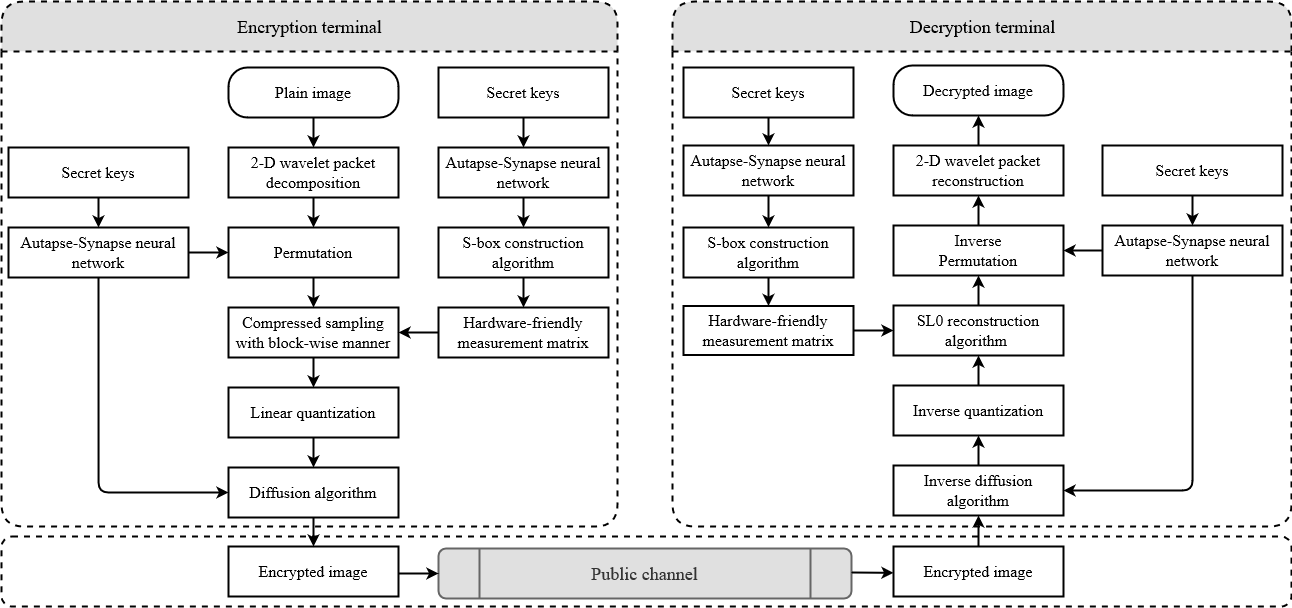
\includegraphics[width=0.5\textwidth]{fig5.png}
		\caption{Workflow of the proposed image cryptosystem}
	\label{fig5}
\end{figure}
 

\textbf{Step 1.} First, to be capable of performing compressed sampling on the plain image $P 1 \in \mathbb{N}^{n \times n}$  through 2-D measurement matrix, it is sparsely represented using the multi-layer wavelet packet decomposition. And the corresponding sparse coefficient matrix is denoted as  $P2 \in \mathbb{R}^{n \times n}$.\\

\textbf{Step 2.} Then, the coefficient matrix $P 2$  is shuffled with good scrambling effect, thereby spreading its principal components uniformly to each column. This process can be elaborated into Eq.\ref{eq10}, where the symbols  $z_{1} \in \mathbb{N}^{n \times n}$ and $z_{2} \in \mathbb{N}^{n \times n}$  are the index sequences generated by sorting the output values of new synapse-autapse memristive neural network model. And the symbol ''mod'' means the modulus operator.

\begin{equation}\label{eq10}
\left\{ {\begin{array}{*{20}{c}}
   {\left[ {\begin{array}{*{20}{c}}
   k  \\
   t  \\
\end{array}} \right] = \bmod \left( {\left[ {\begin{array}{*{20}{c}}
   {{z_{11}}} & {{z_{12}}}  \\
   {{z_{21}}} & {{z_{22}}}  \\
\end{array}} \right] \times \left[ {\begin{array}{*{20}{c}}
   i  \\
   j  \\
\end{array}} \right],\left[ {\begin{array}{*{20}{c}}
   n  \\
   n  \\
\end{array}} \right]} \right)}  \\
   {{P_3}(i,j) = {P_2}(k,t)}  \\
\end{array}} \right. 
\end{equation}
with ${z_{ij}}\,\,(i = 1...2\,;\,j = 1...2)$ defined as ${z_{11}} = 1$; ${z_{12}}={z_1}$; ${z_{21}} = {z_2}$; ${z_{22}} = {z_1}.{z_2} + 1$.\\

\textbf{Step 3.} Next, the proposed memristive autapse-synapse neural network is adopted to construct the S-box following Algorithm \ref{algo1}. Afterward, according to Algorithm \ref{algo2}, the small-scale measurement matrix $\Phi$   consisting of $-1$  and $1$ is obtained. The measurement matrix generated is more hardware friendly than some chaotic measurement matrix and the randomly structured measurement matrix \cite{canh2021restricted}.


\textbf{Step 4.} The matrix  $P3$ is partitioned into several non-overlapping blocks of size  $n/N \times n/N$. Where, $N=n/64$. Then, each block is linearly projected onto the measurement matrix $\Phi$  and the resulting values are concatenated to obtain the compressed matrix  $P4$. Later, it is linearly quantized to the interval $[0,255]$. This process can be expressed as Eq.\ref{eq15}.

\begin{equation}\label{eq15}
P 5=255 \cdot\left(P_{4}-\min \left(P_{4}\right)\right) \cdot\left(\max \left(P_{4}\right)-\min \left(P_{4}\right)\right)^{-1}
\end{equation}



\textbf{Step 5.} Under the control of sequences  $\left\{d_{i}\right\}_{i=1}^{2}$ constructed by new memristive synapse-autapse  neural network model, the compressed image $P5$  is subjected to the bidirectional diffusion to obtain the final encrypted image $C \in \mathbb{N}^{0.5 n \times n}$. This process can be expressed as Eq.\ref{eq16} and Eq.\ref{eq17}, where the vectors  $\left\{s_{i}\right\}_{i=1}^{2}=\left(\left(\left\{d_{i}\right\}_{i=1}^{2}+10\right) \times 10^{10}\right) \bmod 256$.

\begin{equation}\label{eq16}
P 6(i)=\left(P 6(i-1)+P 5(i)+s_{1}(i)\right) \bmod 256
\end{equation}
\begin{equation}\label{eq17}
C(i)=\left(C(i+1)+P 6(i)+s_{2}(i)\right) \bmod 256
\end{equation}


\begin{algorithm}
\KwData{Memristive synapse-autapse neuron model parameters; measurement matrix dimension $(n/2N, n/N)$.}
\KwResult{Measurement matrix $\Phi$.}



\textbf{1.} Initialize an unsigned 8-bit integer variate  $pt$ with size of  $\textit{(1,256)}$, whose elements are all equal to zero.\\
\textbf{2.} Initialize a floating-point variate $phi$, whose elements are all equal to zero.\\
\textbf{3.} $p t=SB\left(\left[e_{0}, f_{0}, g_{0}\right]\right)$


  \For{$i = 1$:$256$}{
	\textbf{4.} $\textit{tmp}=\operatorname{\textit{dec}} 2 \operatorname{\textit{bin}}(pt(i), 8)$;
	
	\textbf{5.} $num=1$
   
   
 \For{$i = 7$:$-1$:$0$}{
	\textbf{6.} \textit{phi} $(8 i-j)=\operatorname{str} 2 \operatorname{\textit{num}}(\operatorname{\textit{tmp}}($ \textit{num} $))$;\\	        
	\textbf{7.} $n u m=n u m+1$;
	}
	}
	
\textbf{8.} Initialize $\Phi=p h i$ and rearrange it as size $(n / 2 N, n / N)$ with column-wise manner.	\\
\textbf{9.} Arrange the element value equal to zero in matrix $\Phi$ to be $-1$.
    
   \caption{Construction of the measurement matrix}\label{algo2}
\end{algorithm}

The encrypted image can be decrypted and decompressed to acquire the accurately reconstructed image with the reverse encryption method as shown in Fig. \ref{fig5}. 

\subsection{Performance evaluation}
This section is devoted to the analysis of the performances of the proposal. First it is important to note that all simulations are performed using a laptop with Intel CoreT M i7 – 4600M, 3.00GHz, 64 bits central processing unit, 8GB RAM. The environment is equipped with MATLAB 2014 running under 64-bits operating system. To analyze the performances of the proposed algorithm three medical images (each of size  $256 \times 256$) are selected from the free medical images data base \textit{MedPix} (\textit{https://medpix.nlm.nih.gov/home}). The proposed memristive autapse-synapse neural network  model is solved (with the parameters of Fig.\ref{fig4}-a) using the fourth-order Runge-Kutta algorithm to yield chaotic sequences useful in the compression-encryption-decryption stages. The algorithm is applied on the test images (each of size  $256 \times 256$) and the results of compression-encryption-decryption-reconstruction is presented on Fig.\ref{fig6} where the first column contains the original input medical data (each of size  $256 \times 256$). The second column contains the compressed encrypted medical data (each of size  $128 \times 256$) . The third column contains the results of decryption-reconstruction. Three observations can emerge from these results. \textbf{(1)} The output of the compression provides images each of size $128 \times 256$ when each inputs images is of size  $256 \times 256$. This simply indicates that the images are compressed along the row dimension. \textbf{(2)} The Output of the encryption process (second column) provides images with no profitable information. This simply indicates that the algorithm is capable to secure the input medical data. \textbf{(3)} The output of the compression-encryption-decryption-reconstruction is identical to the input image with few errors.


\begin{figure}[!t]
	\centering
	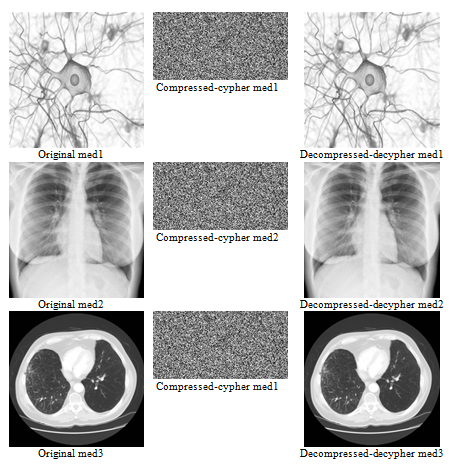
\includegraphics[width=0.5\textwidth]{fig6.png}
		\caption{Results of compression-encryption-decryption-reconstruction processes}
	\label{fig6}
\end{figure}
 
\subsubsection{Histogram analysis}

In image processing, histogram of image refers to the representation of each pixel density with respect to the corresponding gray value. This tool is very useful in image encryption to evaluate some statistical properties of both the plain input data and the output data \cite{njitacke2021complex}. The histogram of the plain input image is randomly distributed. A given encryption algorithm is required to make uniform the distribution of the pixels. Consequently the histogram of the encrypted image is almost uniform. In the present case the first row of  Fig.\ref{fig7} shows the plain image, the compressed-encrypted image and the corresponding histograms. From this result and the above comments it is seen that the proposed algorithm produces output image with uniformly distributed pixels. Consequently the algorithm is secured against statistical attacks.


\begin{figure}[!t]
	\centering
	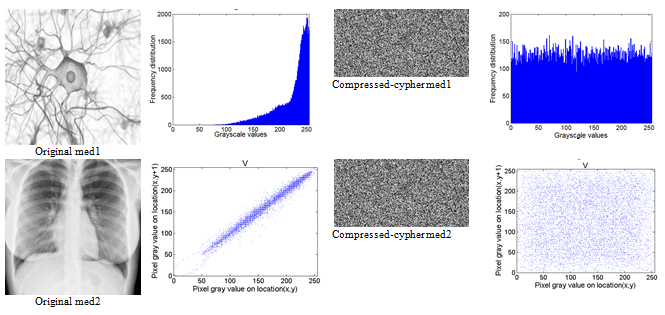
\includegraphics[width=0.5\textwidth]{fig7.png}
		\caption{Original input data with respectve ciphers and the corresponding histograms}
	\label{fig7}
\end{figure}

\subsubsection{Correlation coefficients analysis}

Another efficient tool to evaluate the capability of an algorithm to resist statistical attacks is correlation coefficient \cite{ding2020deepedn}. This metric evaluate how strong is the resemblance between two neighboring pixels in three directions: (horizontal-H, vertical-V and diagonal-D). The results yield a value between $-1$ and $+1$. When the results approach the extreme values ($-1$ or $+1$) this simply indicate very strong correlation between the pixels of the images. Whereas the results close to $0$ indicates very poor correlation between the pixels of the image. The distribution of the correlation between pixels can also be represented along various directions. When the distribution is linear this indicates very high correlation between pixels while there is very poor correlation when the distribution is random. The correlation is computed in cryptography using Eq.\ref{eq20}.

\begin{equation}\label{eq20}
\begin{array}{l}
 {C_{i,j}} = \frac{{A[(i - A(i))(j - A(j))]}}{{\sqrt {B(i)} \sqrt {B(j)} }} \\ 
 with\,\,\,A(i) = \frac{1}{n}\sum\limits_{x = 1}^n {{i_x}} \,\,,\,\,\,B(i) = \frac{1}{n}\sum\limits_{x = 1}^n {{{({i_x} - A(i))}^2}}  \\ 
 \end{array}
\end{equation}

Table \ref{tab5} provides the correlation coefficients of the plain input medical images and the corresponding ciphers. It is observed that for the plain medical images the correlation coefficients are very close to the extreme values ($-1$ or $+1$). This indicates very high correlation between the pixels of the considered data images. In contrast the correlation of the output data are close to zero indicating that the method has destroyed the correlation between the pixels of the plain images. Consequently the proposed algorithm produces data that can resist statistical attacks.

\begin{table}
	\centering
	\caption{Security performances of the proposed work.}
	\label{tab5}
	\resizebox{\columnwidth}{!}{
\begin{tabular}{|c|c|c|c|c|c|c|c|c|}
\hline \multirow{2}{*}{ Test images } & \multicolumn{3}{|c|}{ Correlation coefficients } & \multirow{2}{*}{ Entropy } & NPCR & UACI & PSNR & MSSIM \\
\cline { 2 - 4 } & $\mathrm{H}$ & $\mathrm{V}$ & $\mathrm{D}$ & & $(\%)$ & $(\%)$  & &  \\
\hline Original med1 & $0.9025$ & $0.9000$ & $0.8614$ & $6.4263$ & \multirow{2}{*}{$99.9771$} & $33.4012$ & $38.1747$ & $0.8990$ \\
\cline { 1 - 5 } Compressed-cypher med1 & $0.0004$ & $-0.0002$ & $-0.0007$ & $7.9946$ & &  & & \\
\hline Original med2 & $0.9015$ & $0.8256$ & $0.8125$ & $7.0011$ & \multirow{2}{*}{$99.9901$} & $33.5107$ & $37.4525$ & $0.9716$ \\
\cline { 1 - 5 } Compressed-cypher med2 & $-0.0037$ & $0.0019$ & $-0.0069$ & $7.9947$ & & & & \\
\hline


\hline Original med3 & $0.7264$ & $0.6984$ & $0.9804$ & $7.9851$ & \multirow{2}{*}{$99.8612$} & $33.5107$ & $38.2963$ & $0.9278$ \\
\cline { 1 - 5 } Compressed-cypher med3 & $0.0005$ & $-0.0009$ & $-0.0025$ & $7.9018$ & & & & \\
\hline
\end{tabular}
}
\end{table}

\subsubsection{Compression performance analysis}

Structural Similarity Index Measure ($ S\!S\!I\!M $) and Peack Signal to Noise Ratio ($ P\!S\!N\!R $) are two important metrics exploited to compare the output data of any compression algorithm with respect to its input data \cite{tellez2019neural}. This helps to evaluate the performance of the considered compression algorithm. $ N\!P\!C\!R $ measures in decibels ($ dB $) the ratio between the maximum power of the input signal and the noise introduced by the considered compression operation. In image and video compression, considering 8-bits data, the PSNR should belong to the set $[30\,;\,50]$  to allow human perception.  SSIM measures the degradation of the plain input data in terms of luminance and contrast. Table \ref{tab5} presents the results of $ P\!S\!N\!R $ and $ M\!S\!S\!I\!M $ (Mean $ S\!S\!I\!M $) for the proposed compression algorithm. It is observed that the results are within the threshold values. Consequently the compression-reconstruction processes are effective.

\subsubsection{Entropy analysis}

Entropy is a statistical tool exploited to evaluate the degree of randomness in a given data. In cryptography this metric is exploited to check if the diffusion step of the algorithm is efficient \cite{xu2021invertible}. There exist various type of entropy but global entropy is the most used in cryptography and this type will be exploited in this work.  Given an 8-bits image the global entropy is exploited using Eq.\ref{eq21}. 

\begin{equation}\label{eq21}
GE(i) = \sum\limits_{x = 1}^{{2^n} - 1} {p({i_x}){{\log }_2}\frac{1}{{p({i_x})}}} 
\end{equation}

For 8-bits image the threshold value of the entropy is 8. Eq.\ref{eq21} has been exploited to compute the entropy values for the three medical plain images and the corresponding ciphers. The results are presented in Table \ref{tab5}. From this table it is observed that the entropy scores of cipher is around the threshold value 8 compare to the entropy values of the plain input images. Consequently the proposed algorithm can resist unauthorized intrusion.

\subsubsection{NPCR and UACI analyses}

NPCR and UACI are two metrics exploited to quantify the capability of the memristive autapse-synapse based method to resist differential attacks \cite{xu2021invertible}. In such intrusion unauthorized party create one pixel difference in the image and exploit this difference to obtain the acquaintance between the plain input and the corresponding cipher image. Considering a plain image and the corresponding cipher, The $ N\!P\!C\!R $ and the $ U\!A\!C\!I $  can be obtained as the cipher of the same plain image with just one different pixel.  And these metrics are usually computed using Eq.\ref{eq22} and Eq.\ref{eq23}.

\begin{equation}\label{eq22}
U\!A\!C\!I = \frac{{100}}{{xy}}\sum\limits_{i = 1}^x {\sum\limits_{j = 1}^y {\frac{{\left| {{C_{{r_2}}}(i,j) - {C_{{r_1}}}(i,j)} \right|}}{{255}}} } 
\end{equation}

\begin{equation}\label{eq23}
\begin{array}{l}
\,\,\,\,\,\,\,\,\,\,\,\,\,\,\,\,\,\,\,\,\,\,\,\, N\!P\!C\!R = \frac{{100}}{{xy}}\sum\limits_{i = 1}^x {\sum\limits_{j = 1}^y {Diff(i,j)} } \,\,; \\ 
\\
 where\,\,Diff(i,j) = \left\{ \begin{array}{l}
 1\,\,\,for\,\,{C_{{r_1}}}(i,j) \ne {C_{{r_2}}}(i,j) \\ 
 0\,\,for\,\,{C_{{r_1}}}(i,j) = {C_{{r_2}}}(i,j) \\ 
 \end{array} \right. \\ 
 \end{array}
\end{equation}


represents the size of the image. The threshold value of the NPCR is 100\% while the threshold value of the UACI is 33.6\%. Eq.\ref{eq22} and Eq.\ref{eq23} have been exploited in this work to compute both $ N\!P\!C\!R $ and $ U\!A\!C\!I $. The outcomes are shown in Table \ref{tab5} from where the results are very close to the threshold values. This simply indicates that the proposed algorithm can resist differential attack.   


%\begin{table}
%	\centering
%	\caption{Comparative results.}
%	\label{tab6}
%	\resizebox{\columnwidth}{!}{
%\begin{tabular}{|c|c|c|c|c|c|c|c|}
%\hline Test images & MSSIM & PSNR & Entropy & NPCR (\%) & UACI (\%) & Enc. Time & Dec. Time \\
%\hline \cite{wang2019visually} & $0.9903$ & $31.7986$ & $7.9884$ & $99.8700$ & $33.4027$ & $0.1544$ & $2.2489$ \\
%\hline \cite{zhang2022high} & $0.9853$ & $38.2045$ & $7.9245$ & $99.2410$ & $33.1542$ & $1.5308$ & $3.5124$ \\
%\hline \cite{ren2022visually} & $0.9970$ & $35.4988$ & $7.9896$ & $99.0589$ & $33.3571$ & $2.1296$ & $6.7961$ \\
%\hline \cite{huang2022visually} & $0.9950$ & $38.2105$ & $7.9900$ & $99.9854$ & $33.4602$ & $0.260829$ & $3.0218$ \\
%\hline This work & $0.9971$ & $38.2963$ & $99.9901$ & $99.9901$ & $33.5820$ & $0.1384$ & $1.5144$ \\
%\hline
%\end{tabular}
%}
%\end{table}


\section{Conclusion}
\label{con}
The dynamics of two different neurons, coupled with both memristive synapse and memristive autapse, was first considered in this work. Then using Lyapunov exponent, bifurcation, Kaplan-York dimension and phase portrait as dynamical analysis methods, it was established that the model is capable  of displaying various windows of both chaotic and periodic attractors with the variation of the coupling strength. Afterward, the S-box controlled by the coupled memristive neuron model has been exploited in chaotic windows to construct a hardware-friendly measurement matrix for medical image compression, followed by a series of encryption procedures. Ultimately, it can be concluded from the extensive experimental results and analysis that the proposed medical data protection scheme is secure enough and can be useful in real applications.


\bibliographystyle{IEEEtran}
%\bibliographystyle{}
% argument is your BibTeX string definitions and bibliography database(s)
\bibliography{Bibliography}


\end{document}


